\section{Experimental Results}
\label{sec:experiments}

\subsection{Experimental Setting}

We conducted a reproducible pilot study using a three-stage, three-product discrete-event simulator. The simulator represents interstage WIP, finished-product inventory, backlog, sequence-dependent cleaning, stochastic demand, equipment availability, and yield. Table~\ref{tab:experimental-setting} summarizes the experimental conditions. Complete trajectories, rather than overlapping windows, were assigned to the training, validation, and test sets. All closed-loop policies were evaluated using common random numbers.

\begin{table}[t]
  \centering
  \caption{Experimental conditions.}
  \label{tab:experimental-setting}
  \small
  \begin{tabular}{p{0.30\columnwidth}p{0.55\columnwidth}}
    \hline
    Item & Setting \\
    \hline
    Production system & 3 stages and 3 products \\
    Uncertainty & Demand, availability, yield, and cleaning time \\
    Data split & 30/12/18 training/validation/test trajectories \\
    Trajectory length & 32 periods \\
    TCN input window & 12 periods \\
    Surrogate test & Nominal training and OOD stress testing; 3 seeds \\
    Closed-loop test & 5 paired replications per condition; 15 periods \\
    Planning model & 3-period horizon; 2 scenarios \\
    MILP solver & CBC; 10-s time limit \\
    \hline
  \end{tabular}
\end{table}

The surrogate baselines were a current-state MLP, a flattened-window MLP, and a data-only TCN. These were compared with the physics-informed TCN and its piecewise-affine (PWA) approximation. For closed-loop evaluation, the proposed scenario rolling-horizon policy was compared with a setup-aware heuristic, deterministic rolling-horizon planning, and scenario block planning.

\subsection{Surrogate Accuracy and PWA Approximation}

Figure~\ref{fig:temporal-physics} separates the contributions of temporal convolution and physics-informed training. The data-only TCN achieved a mean throughput NRMSE of 0.225 and a multi-period WIP NRMSE of 0.221. Its WIP error was 27.0\% lower than that of the current-state MLP and 31.6\% lower than that of the parameter-matched window MLP. Thus, the improvement cannot be attributed only to the availability of lagged inputs. Physics-informed training retained similar predictive accuracy (throughput NRMSE 0.220) while reducing the violation rate at low-WIP, low-availability, and high-cleaning OOD points from 36.4\% to 6.5\%. Monotonicity violations decreased from 6.4\% to 2.7\%.

\begin{figure*}[t]
  \centering
  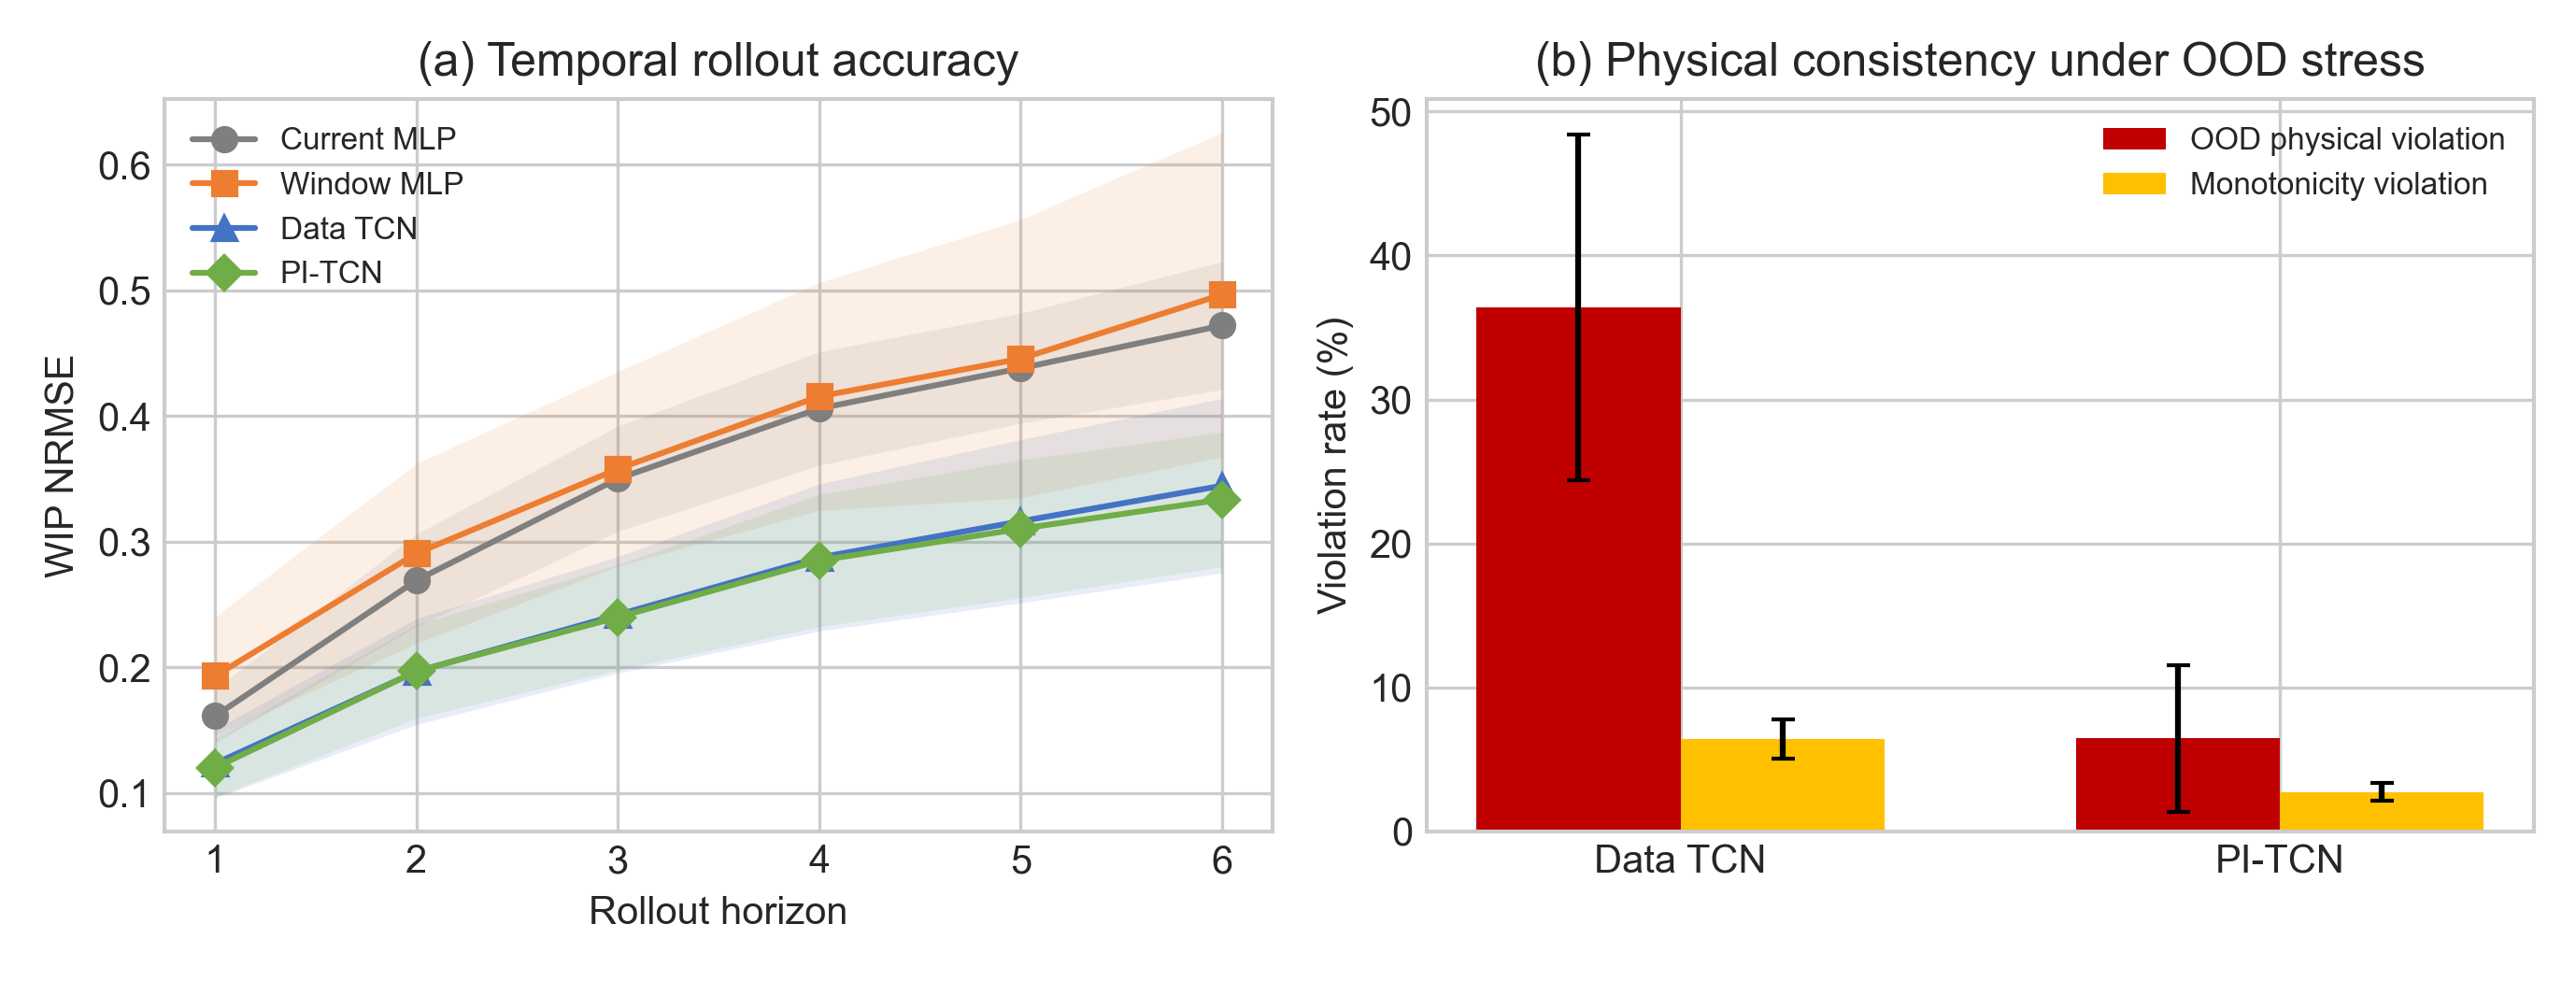
\includegraphics[width=0.92\textwidth]{experiments/output_temporal_final/temporal_physics_evidence.png}
  \caption{Independent evaluation of (a) temporal rollout accuracy and (b) physical consistency under OOD stress. Lines and bars show means over three training seeds and three stages; shaded areas and error bars denote 95\% intervals.}
  \label{fig:temporal-physics}
\end{figure*}

\subsection{Closed-Loop Planning Performance}

Figure~\ref{fig:closed-loop-cost} compares the policies using realized outcomes from the high-fidelity simulator. With a 10-s MILP limit, scenario rolling-horizon control achieved the lowest mean objective value (8319), compared with scenario block planning (8364) and deterministic rolling-horizon planning (8400). Its fill rate was 0.358, versus 0.346 and 0.329, respectively. Relative to scenario block planning, it reduced mean WIP from 30.1 to 29.2 and cleaning time from 7.7 to 7.2. Relative to the setup-aware heuristic, it reduced the objective value by 17.4\%, mean WIP by 74.8\%, and cleaning time by 69.8\%. The mean run-level 95th-percentile solution time was 9.49~s, and all scenario rolling-horizon solves returned an accepted feasible status. Because the paired confidence intervals against deterministic and block planning included zero, these differences should be interpreted as pilot evidence rather than conclusive statistical superiority.

\begin{figure*}[t]
  \centering
  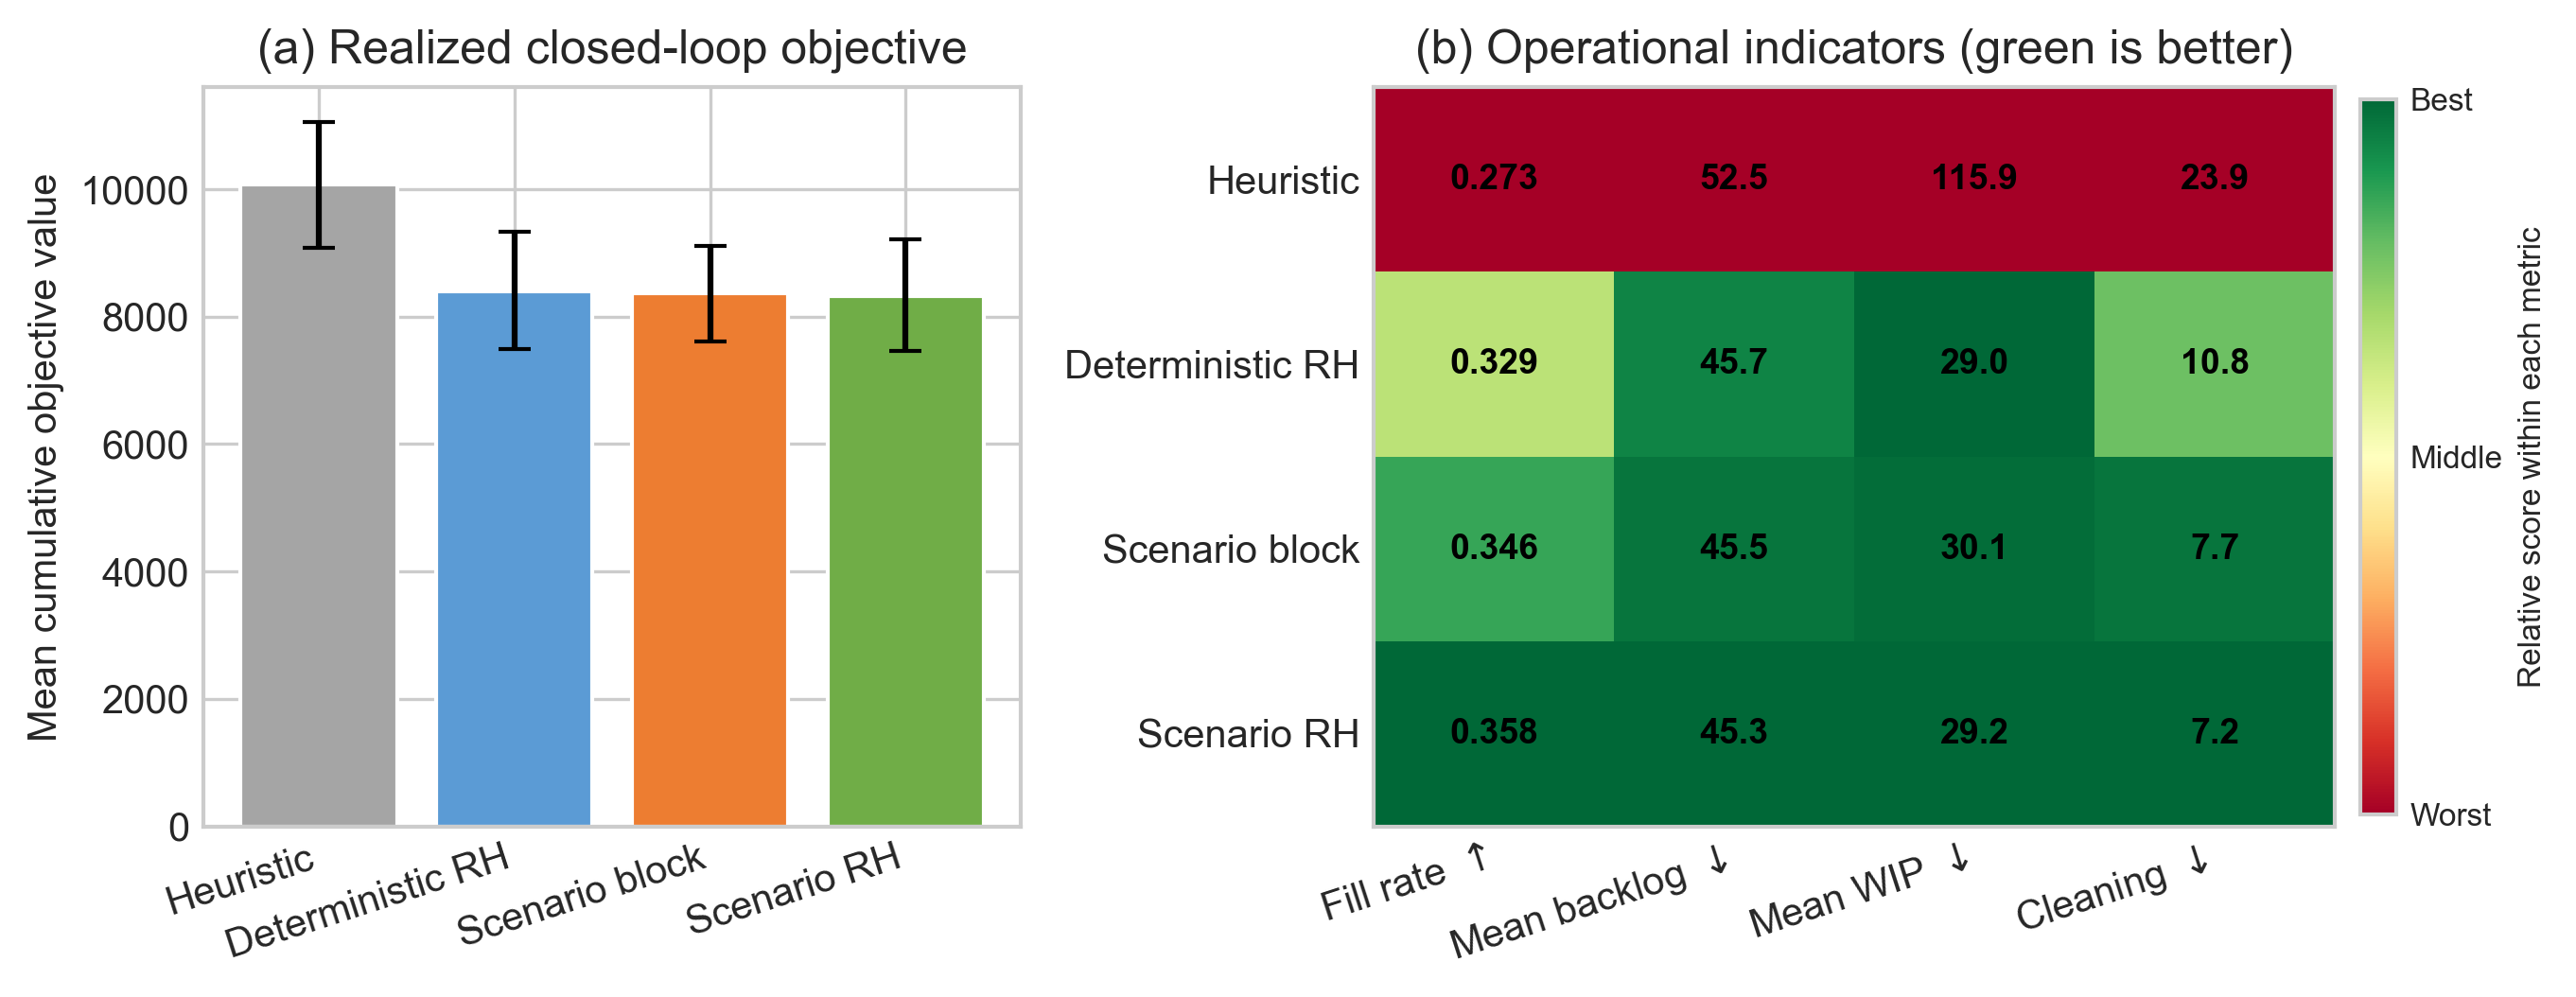
\includegraphics[width=0.92\textwidth]{experiments/output_10s/operational_performance.png}
  \caption{Closed-loop operational performance: (a) realized cumulative objective value with 95\% bootstrap intervals and (b) four indicators computed uniformly for all policies. The color scale is normalized separately within each metric from the worst (red, 0) to the best (green, 1) of the four policies; it does not represent an absolute performance threshold. Cell labels report the original values.}
  \label{fig:closed-loop-cost}
\end{figure*}
